\chapter{\leavevmode\newline Motivation and Research Objective}
\label{chap:chapter_2}

The research objective of the truck trailer wheel robot (TTWR) system is to harness the potential of model-based deep reinforcement learning to achieve end-to-end control, with a focus on enhancing efficiency, stability, and real-world applicability. The main goals and key components of this research include:
\begin{enumerate}
   \item Building Trailer Movement State Equations: Developing precise mathematical models to represent the state dynamics of the TTWR system. This foundational work will create a framework for subsequent control and planning algorithms.
   \item Comparison of Classical Path Planning Methods: Investigating and comparing different classical path planning methods, including:
   \begin{itemize}
     \item Polynomial curve: One of the most simple and popular methods used in nowadays industrial and research field due to its computational efficiency and robust performance, it also provides a flexible framework that can be easily adapted to various requirements
     \item Clothoid curve: Providing smooth transitions between curves of different curvatures, which property makes it an ideal choice for applications such as road design, robotics, and autonomous vehicle navigation, where smooth and continuous paths are often desired.
     \item Dubins curve: Exploring its applicability for smooth path generation. The popularity of this algorithm is because of its simplicity and analytical tractability, and the algorithm also considers the physical constraints of the vehicle, such as its minimum turning radius.
     \item A* search: Analyzing its efficiency in finding optimal paths in complex environments. The A* search is an extension of Dijkstra's algorithm, with the added capability of using a heuristic to estimate the cost from the current node to the goal, allowing it to find optimal paths more efficiently.
   \end{itemize}
   \item Comparison of Different Control Algorithms: Conducting a comparative study of different control algorithms to identify the most effective approach for the TTWR system, including:
   \begin{itemize}
     \item PID: Evaluating its robustness and simplicity. Although PID controllers are simple, well-understood, and widely used in various industries,and hey are computationally efficient and work well for systems with known and stable dynamics, the tuning of PID parameters can be challenging, especially for complex or nonlinear systems. PID controllers may not handle disturbances or model uncertainties well, and they may require manual re-tuning if system dynamics change.
     \item LQR: Assessing its ability to handle nonlinear TTWR systems. Because LQR is mainly optimal for linear systems, providing robust performance by minimizing a quadratic cost function. It can handle multi-input and multi-output systems and can be designed to meet specific performance criteria. But when for nonlinear model, the lionization will cause inaccuracy because the LQR algorithm requires a precise mathematical model of the system and assumes linearity, moreover, designing and solving the underlying optimization problem can be computationally intensive.
     \item MPC: Analyzing its potential to handle constraints and model nonlinearities. The advantage of MPC is that the consideration of future states by solving an optimization problem at each step, allowing it to handle constraints and adapt to changes in system dynamics. But it requires a detailed mathematical model and can be computationally demanding, especially for high-frequency or real-time applications. The optimization problem must be solved at each time step, which may lead to challenges in implementation and tuning.
   \end{itemize}
   \item Implementation of Model-Free Reinforcement Learning: Implementing and evaluating different model-free reinforcement learning algorithms, such as:
   \begin{itemize}
     \item DQN: Investigating its effectiveness in discrete action spaces. DQN combines Q-learning with deep neural networks, enabling the handling of high-dimensional input spaces. It's robust and has been successfully applied to various tasks, especially in discrete action spaces. However, the continuous action spaces and instability during will be a problem in real world scenario training. The experience replay buffer required can be memory-intensive.
     \item DDPG: DDPG extends the ideas of DQN to continuous action spaces by combining Q-learning with policy gradients. It has shown success in various complex environments. But DDPG can be sensitive to hyperparameters and might suffer from training instability. It requires careful tuning and normalization techniques to achieve optimal performance.
     \item TD3: Assessing its ability to achieve stable learning in complex environments. TD3 improves upon DDPG by addressing overestimation bias and instability. It introduces a clipped double-Q learning and delayed policy updates, leading to more stable and efficient training. TD3, while more stable than DDPG, still requires careful hyperparameter tuning. The additional complexity in the algorithm might increase the implementation difficulty compared to simpler methods like DQN.
   \end{itemize}
   \item Implementation of Model-Based Reinforcement Learning: Implementing and evaluating different model-based reinforcement learning algorithms, such as:
   \begin{itemize}
     \item MBRL with known model \cite{sprayberry2023data}: where we plan over a known model, and only use learning for the global solution. The learnt model is based on classical trajectory planning including A*, RRT, or Dubins path, and after integrated with TTWR physical model, the model will generate TTWR trajectory states for the controller to take as input. The model-free RL algorithm will be used for the agent to interact with the environment, which is shown in figure \ref{fig: MBRL based on known model}
     \item Model-based RL with a learned model, where we both learn a model and learn a global solution.
   \end{itemize}
\end{enumerate}

\begin{figure}[h]
\centering
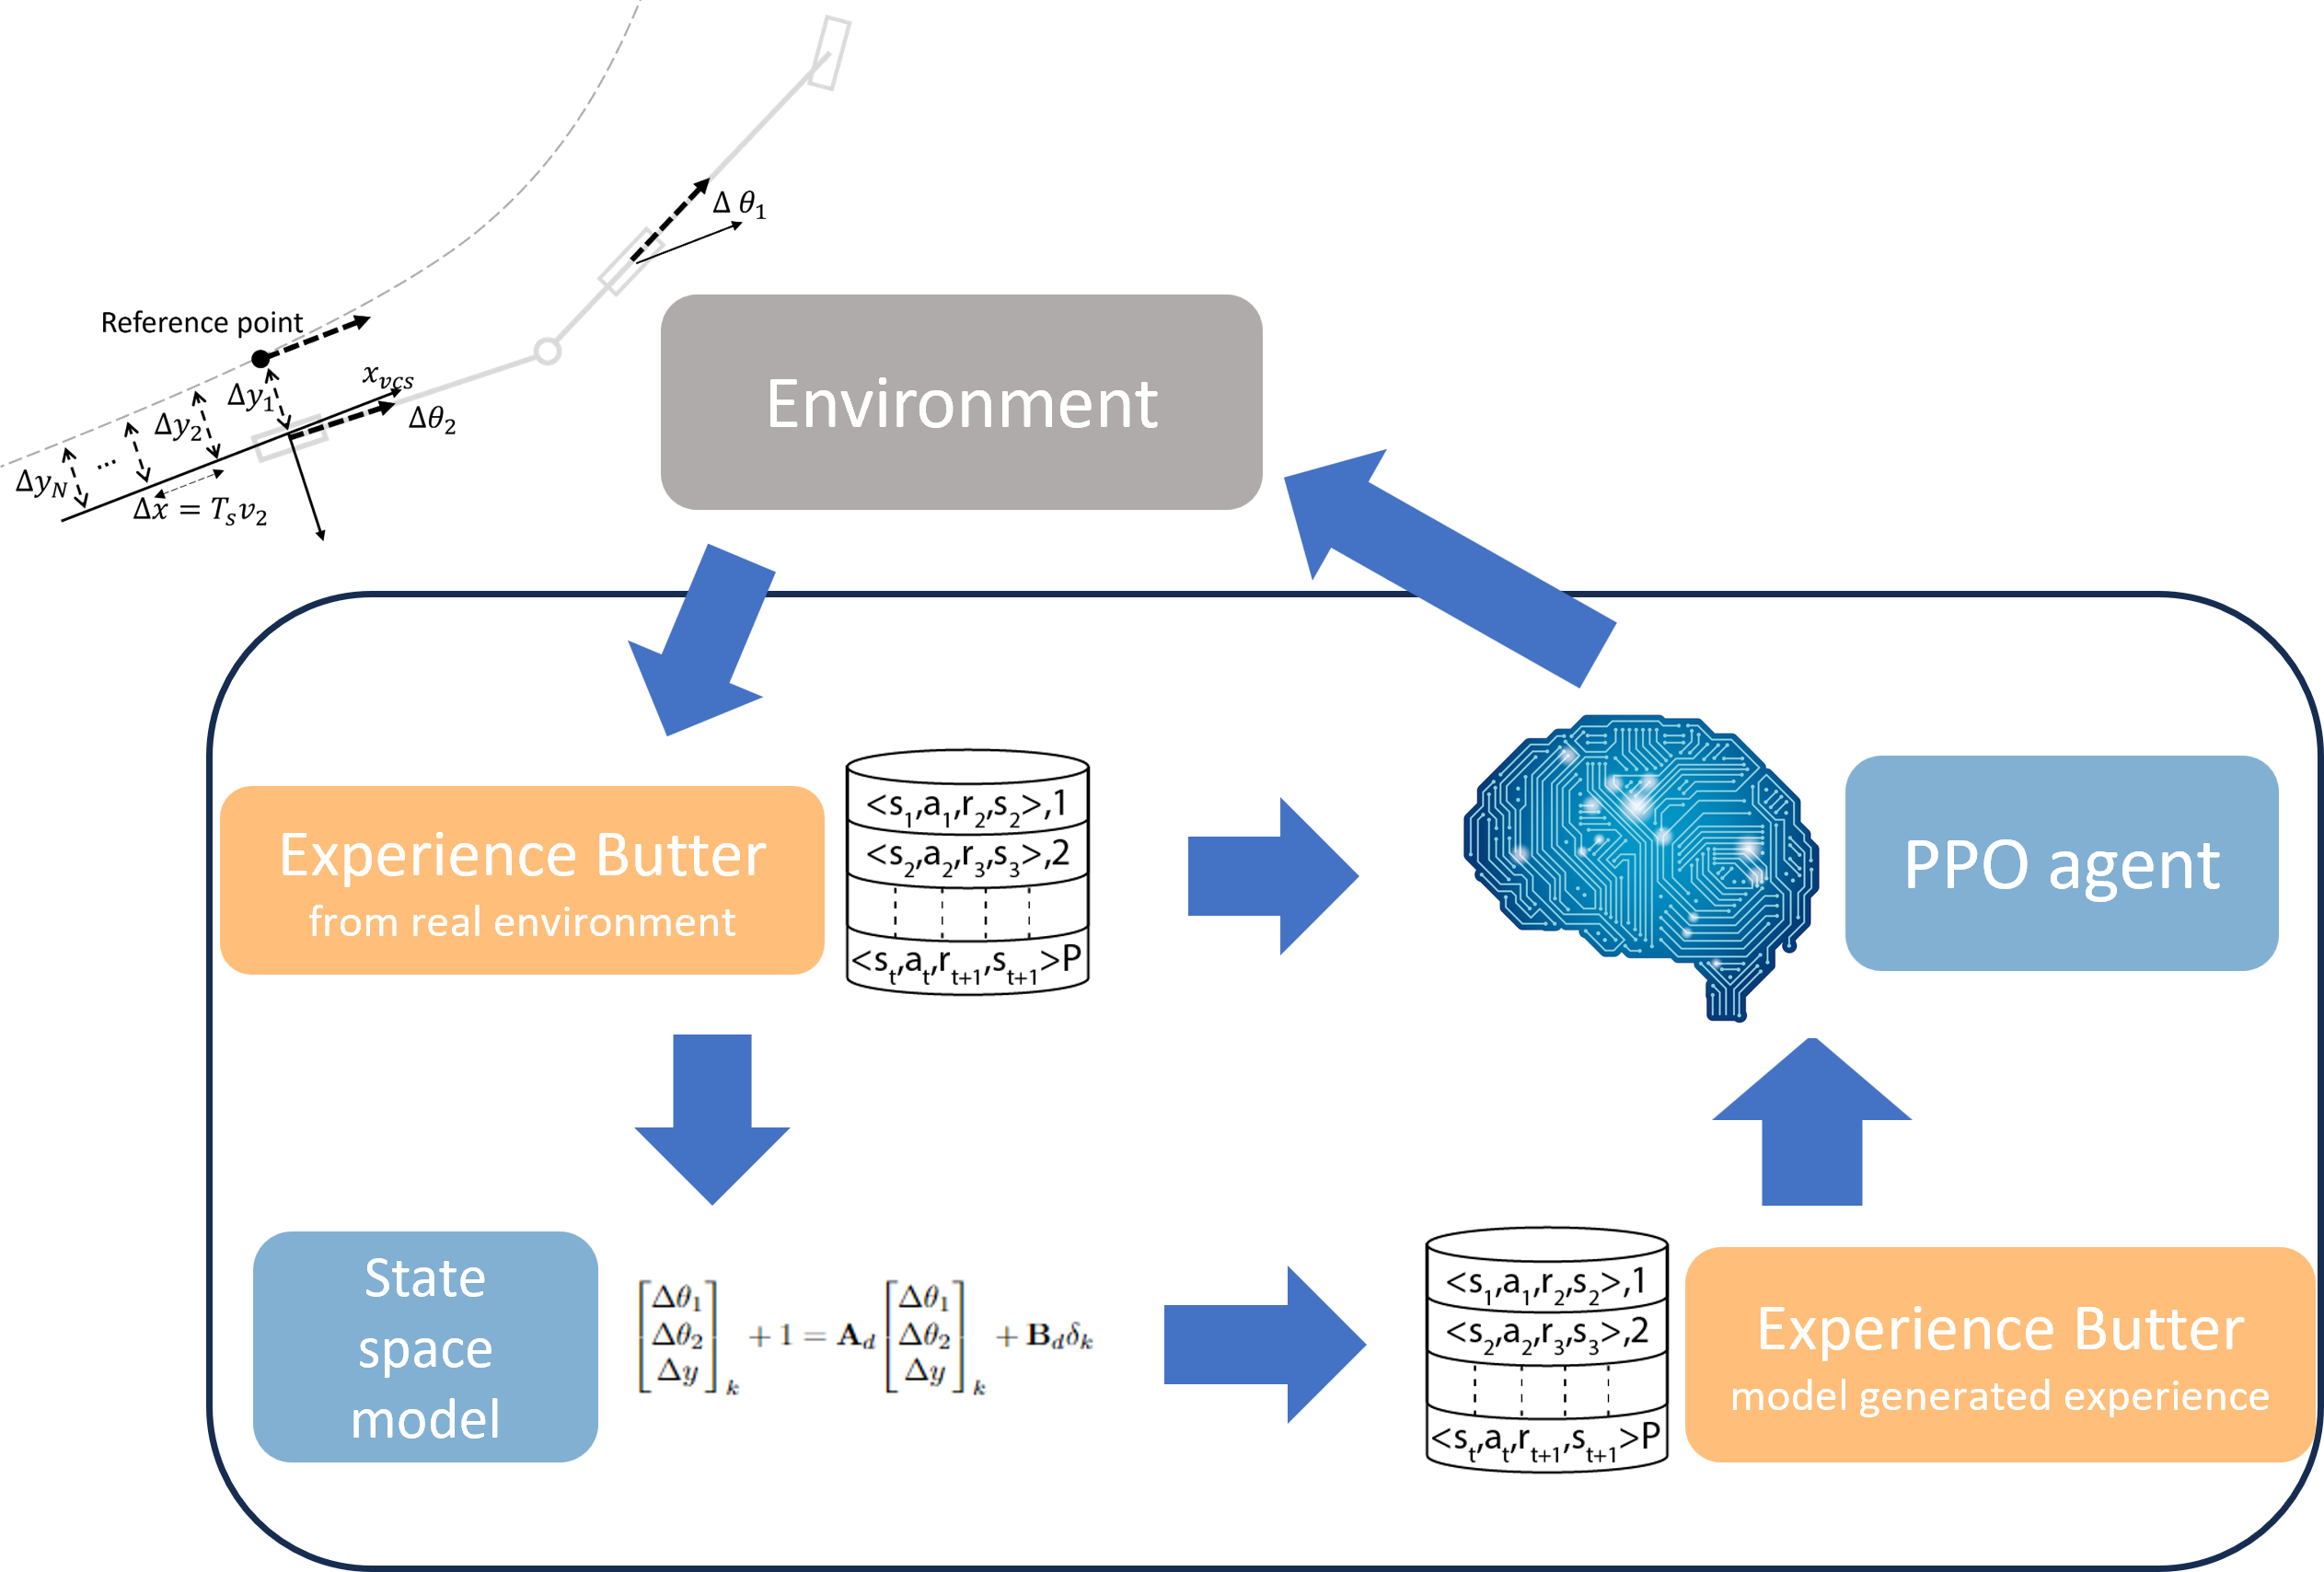
\includegraphics[width=0.8\linewidth]{fig/known mbrl schema.png}
\caption{MBRL based on known model}
\label{fig: MBRL based on known model}
\end{figure}

The proposed research aims to introduce a noval approach using model-based reinforcement learning for end-to-end control in truck-trailer wheel robot systems. While this is an exciting direction, it comes with its own challenges:

\begin{enumerate}
   \item World State Representation: Effectively representing the world states, including surrounding objects, system states, and movement cost, is a complex task that requires innovative methods to capture all relevant information without overwhelming the computational resources.
   \item Stability of Reinforcement Learning Algorithm: Ensuring the stability of the reinforcement learning algorithm, especially in the face of non-stationary and unpredictable real-world scenarios, is a critical challenge. Fine-tuning the balance between exploration and exploitation and devising robust training techniques will be essential.
   \item Computational Efficiency in Complex Environments: Designing computationally efficient methods that can be deployed in complex real-world environments without sacrificing performance or safety is a significant hurdle. Developing lightweight models and optimizing computation will be key to the successful implementation of the TTWR system.
\end{enumerate}

This research aims to make significant improvements in the control and automation of TTWR systems. By tackling the challenges and focusing on modern AI-based solutions, the goal is to enhance safety, efficiency, and adaptability in autonomous vehicles and complex robotic systems. The success of this work could lead to practical applications that are more responsive and reliable, improving efficiency of daily transportation and optimize energy usage.